\documentclass[11pt,compress,t,notes=noshow, xcolor=table]{beamer}
\usepackage[]{graphicx}\usepackage[]{color}
% maxwidth is the original width if it is less than linewidth
% otherwise use linewidth (to make sure the graphics do not exceed the margin)
\makeatletter
\def\maxwidth{ %
  \ifdim\Gin@nat@width>\linewidth
    \linewidth
  \else
    \Gin@nat@width
  \fi
}
\makeatother

\definecolor{fgcolor}{rgb}{0.345, 0.345, 0.345}
\newcommand{\hlnum}[1]{\textcolor[rgb]{0.686,0.059,0.569}{#1}}%
\newcommand{\hlstr}[1]{\textcolor[rgb]{0.192,0.494,0.8}{#1}}%
\newcommand{\hlcom}[1]{\textcolor[rgb]{0.678,0.584,0.686}{\textit{#1}}}%
\newcommand{\hlopt}[1]{\textcolor[rgb]{0,0,0}{#1}}%
\newcommand{\hlstd}[1]{\textcolor[rgb]{0.345,0.345,0.345}{#1}}%
\newcommand{\hlkwa}[1]{\textcolor[rgb]{0.161,0.373,0.58}{\textbf{#1}}}%
\newcommand{\hlkwb}[1]{\textcolor[rgb]{0.69,0.353,0.396}{#1}}%
\newcommand{\hlkwc}[1]{\textcolor[rgb]{0.333,0.667,0.333}{#1}}%
\newcommand{\hlkwd}[1]{\textcolor[rgb]{0.737,0.353,0.396}{\textbf{#1}}}%
\let\hlipl\hlkwb

\usepackage{framed}
\makeatletter
\newenvironment{kframe}{%
 \def\at@end@of@kframe{}%
 \ifinner\ifhmode%
  \def\at@end@of@kframe{\end{minipage}}%
  \begin{minipage}{\columnwidth}%
 \fi\fi%
 \def\FrameCommand##1{\hskip\@totalleftmargin \hskip-\fboxsep
 \colorbox{shadecolor}{##1}\hskip-\fboxsep
     % There is no \\@totalrightmargin, so:
     \hskip-\linewidth \hskip-\@totalleftmargin \hskip\columnwidth}%
 \MakeFramed {\advance\hsize-\width
   \@totalleftmargin\z@ \linewidth\hsize
   \@setminipage}}%
 {\par\unskip\endMakeFramed%
 \at@end@of@kframe}
\makeatother

\definecolor{shadecolor}{rgb}{.97, .97, .97}
\definecolor{messagecolor}{rgb}{0, 0, 0}
\definecolor{warningcolor}{rgb}{1, 0, 1}
\definecolor{errorcolor}{rgb}{1, 0, 0}
\newenvironment{knitrout}{}{} % an empty environment to be redefined in TeX

\usepackage{alltt}
\newcommand{\SweaveOpts}[1]{}  % do not interfere with LaTeX
\newcommand{\SweaveInput}[1]{} % because they are not real TeX commands
\newcommand{\Sexpr}[1]{}       % will only be parsed by R



\usepackage[english]{babel}
\usepackage[utf8]{inputenc}

\usepackage{dsfont}
\usepackage{verbatim}
\usepackage{amsmath}
\usepackage{amsfonts}
\usepackage{bm}
\usepackage{csquotes}
\usepackage{multirow}
\usepackage{longtable}
\usepackage{booktabs}
\usepackage{enumerate}
\usepackage[absolute,overlay]{textpos}
\usepackage{psfrag}
\usepackage{algorithm}
\usepackage{algpseudocode}
\usepackage{eqnarray}
\usepackage{arydshln}
\usepackage{tabularx}
\usepackage{placeins}
\usepackage{tikz}
\usepackage{setspace}
\usepackage{colortbl}
\usepackage{mathtools}
\usepackage{wrapfig}
\usepackage{bm}
\usetikzlibrary{shapes,arrows,automata,positioning,calc,chains,trees, shadows}
\tikzset{
  %Define standard arrow tip
  >=stealth',
  %Define style for boxes
  punkt/.style={
    rectangle,
    rounded corners,
    draw=black, very thick,
    text width=6.5em,
    minimum height=2em,
    text centered},
  % Define arrow style
  pil/.style={
    ->,
    thick,
    shorten <=2pt,
    shorten >=2pt,}
}
\usepackage{subfig}


% Defines macros and environments
\usepackage{bbm}
% basic latex stuff
\newcommand{\pkg}[1]{{\fontseries{b}\selectfont #1}} %fontstyle for R packages
\newcommand{\lz}{\vspace{0.5cm}} %vertical space
\newcommand{\dlz}{\vspace{1cm}} %double vertical space
\newcommand{\oneliner}[1] % Oneliner for important statements
{\begin{block}{}\begin{center}\begin{Large}#1\end{Large}\end{center}\end{block}}


%new environments
\newenvironment{vbframe}  %frame with breaks and verbatim
{
 \begin{frame}[containsverbatim,allowframebreaks]
}
{
\end{frame}
}

\newenvironment{vframe}  %frame with verbatim without breaks (to avoid numbering one slided frames)
{
 \begin{frame}[containsverbatim]
}
{
\end{frame}
}

\newenvironment{blocki}[1]   % itemize block
{
 \begin{block}{#1}\begin{itemize}
}
{
\end{itemize}\end{block}
}

\newenvironment{fragileframe}[2]{  %fragile frame with framebreaks
\begin{frame}[allowframebreaks, fragile, environment = fragileframe]
\frametitle{#1}
#2}
{\end{frame}}


\newcommand{\myframe}[2]{  %short for frame with framebreaks
\begin{frame}[allowframebreaks]
\frametitle{#1}
#2
\end{frame}}

\newcommand{\remark}[1]{
  \textbf{Remark:} #1
}

\newcommand{\citebutton}[2]{%
\NoCaseChange{\resizebox{!}{9pt}{\protect\beamergotobutton{\href{#2}{#1}}}}%
}



\newenvironment{deleteframe}
{
\begingroup
\usebackgroundtemplate{\includegraphics[width=\paperwidth,height=\paperheight]{../style/color/red.png}}
 \begin{frame}
}
{
\end{frame}
\endgroup
}
\newenvironment{simplifyframe}
{
\begingroup
\usebackgroundtemplate{\includegraphics[width=\paperwidth,height=\paperheight]{../style/color/yellow.png}}
 \begin{frame}
}
{
\end{frame}
\endgroup
}\newenvironment{draftframe}
{
\begingroup
\usebackgroundtemplate{\includegraphics[width=\paperwidth,height=\paperheight]{../style/color/green.jpg}}
 \begin{frame}
}
{
\end{frame}
\endgroup
}
% https://tex.stackexchange.com/a/261480: textcolor that works in mathmode
\makeatletter
\renewcommand*{\@textcolor}[3]{%
  \protect\leavevmode
  \begingroup
    \color#1{#2}#3%
  \endgroup
}
\makeatother


%\usetheme{lmu-lecture}
\newcommand{\titlefigure}{figure/cart_tuning_ad_4.pdf}
\newcommand{\learninggoals}{
\item Understand the idea of model based optimization
\item Be able to explein the terms 'surrogate model' and 'expected improvement'
\item Understand the idea of hyperband}
\usepackage{../../style/lmu-lecture}

\let\code=\texttt
\let\proglang=\textsf

\setkeys{Gin}{width=0.9\textwidth}

\title{Introduction to Machine Learning}
% \author{Bernd Bischl, Christoph Molnar, Daniel Schalk, Fabian Scheipl}
\institute{\href{https://compstat-lmu.github.io/lecture_i2ml/}{compstat-lmu.github.io/lecture\_i2ml}}
\date{}

\setbeamertemplate{frametitle}{\expandafter\uppercase\expandafter\insertframetitle}



\begin{document}

  % Load all R packages and set up knitr

% This file loads R packages, configures knitr options and sets preamble.Rnw as parent file
% IF YOU MODIFY THIS, PLZ ALSO MODIFY setup.Rmd ACCORDINGLY...







  
  %! includes: tuning-tuningproblem

\lecturechapter{Hyperparameter Tuning - Advanced Tuning Techniques: MBO \& Hyperband}
\lecture{Introduction to Machine Learning}
\sloppy

\begin{vbframe}{Model-based Optimization}

Model-based optimization (MBO) is a sequential optimization procedure. We start with an initial design, i.e., a set of configurations $\lambda_i$ where we have evaluated the corresponding (resampling) performance. 

Repeat:
  \begin{enumerate}
\item From the available performance measurements, we build a \textbf{surrogate model} that models the relationship between model hyperparameters and estimated generalization error. It serves as a cheap approximation of the expensive objective. 
\item Based on information provided by the surrogate model, a new configuration $\lambda^{(\text{new})}$ is proposed: we pick a value for which the surrogate model predicts a large potential improvement over the already evaluated configurations.
\item The resampling performance of the learner with hyperparameter setting $\lambda^{(\text{new})}$ is evaluated and added to the set of design points.  
\end{enumerate}

\framebreak 

\begin{knitrout}\scriptsize
\definecolor{shadecolor}{rgb}{0.969, 0.969, 0.969}\color{fgcolor}

{\centering 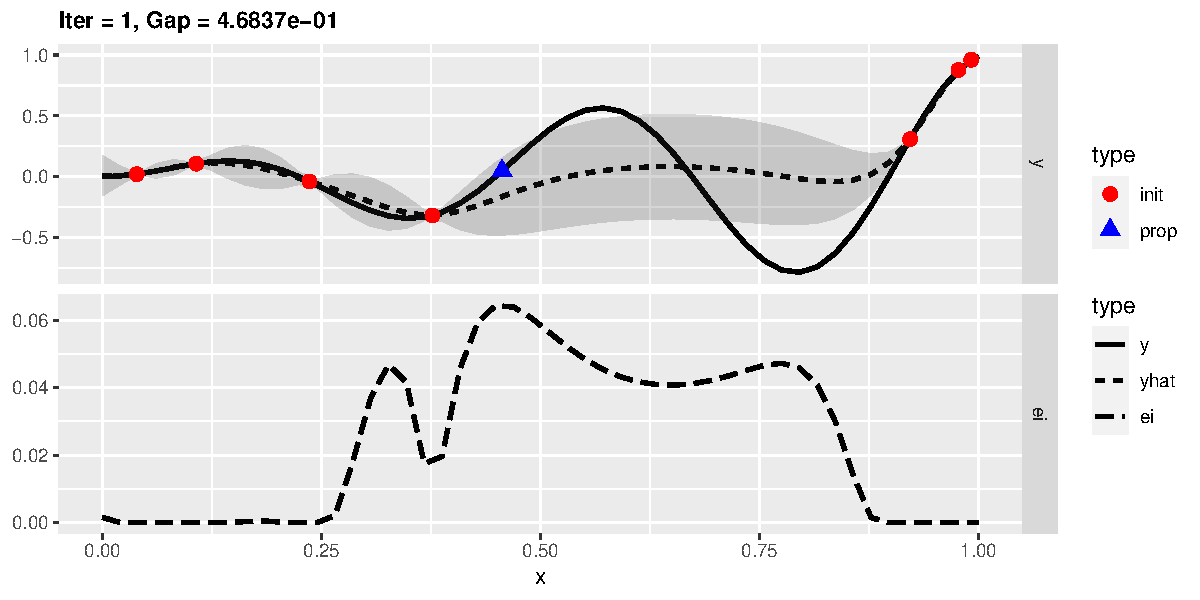
\includegraphics[width=0.95\textwidth]{figure/cart_tuning_ad_1.pdf} 

}



\end{knitrout}
  
  \begin{footnotesize}
Upper plot: The surrogate model (black, dashed) models the \emph{unknown} relationship between input and output (black, solid) based on the initial design (red points).\\
Lower plot: Mean and variance of the surrogate model are used to derive the expected improvement (EI) criterion. The point that maximizes the EI is proposed (blue point). 
\end{footnotesize}

\framebreak 

\begin{knitrout}\scriptsize
\definecolor{shadecolor}{rgb}{0.969, 0.969, 0.969}\color{fgcolor}

{\centering 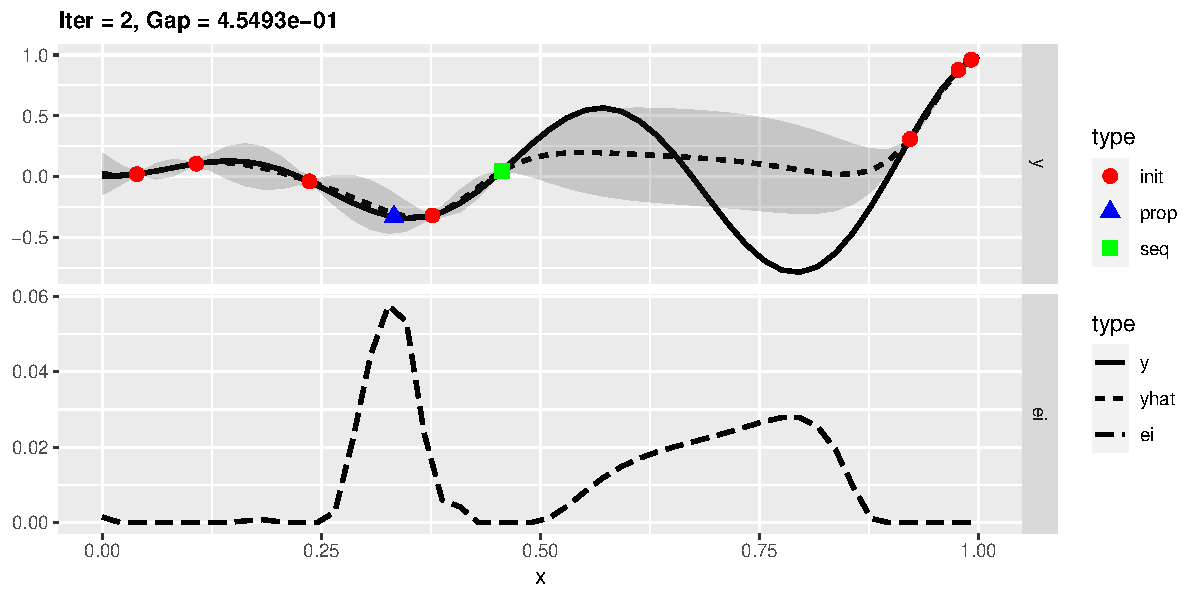
\includegraphics[width=0.95\textwidth]{figure/cart_tuning_ad_2.pdf} 

}



\end{knitrout}
  \begin{footnotesize}
Upper plot: The surrogate model (black, dashed) models the \emph{unknown} relationship between input and output (black, solid) based on the initial design (red points).\\
Lower plot: Mean and variance of the surrogate model are used to derive the expected improvement (EI) criterion. The point that maximizes the EI is proposed (blue point). 
\end{footnotesize}
\framebreak

\begin{knitrout}\scriptsize
\definecolor{shadecolor}{rgb}{0.969, 0.969, 0.969}\color{fgcolor}

{\centering 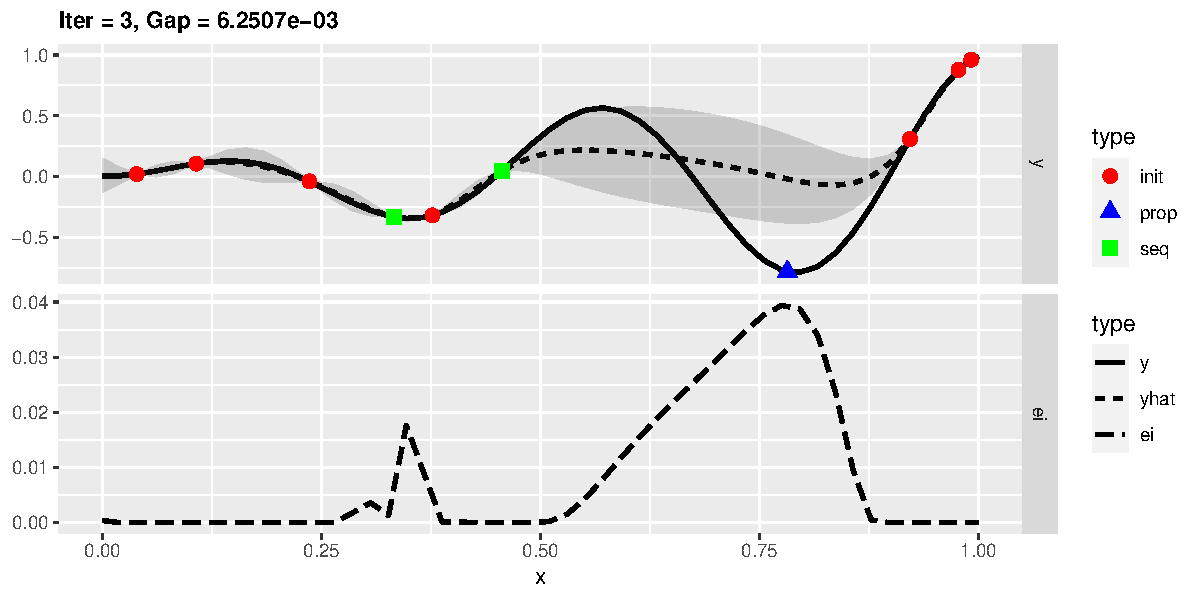
\includegraphics[width=0.95\textwidth]{figure/cart_tuning_ad_3.pdf} 

}



\end{knitrout}
  \begin{footnotesize}
Upper plot: The surrogate model (black, dashed) models the \emph{unknown} relationship between input and output (black, solid) based on the initial design (red points).\\
Lower plot: Mean and variance of the surrogate model are used to derive the expected improvement (EI) criterion. The point that maximizes the EI is proposed (blue point). 
\end{footnotesize}
\framebreak

\begin{knitrout}\scriptsize
\definecolor{shadecolor}{rgb}{0.969, 0.969, 0.969}\color{fgcolor}

{\centering 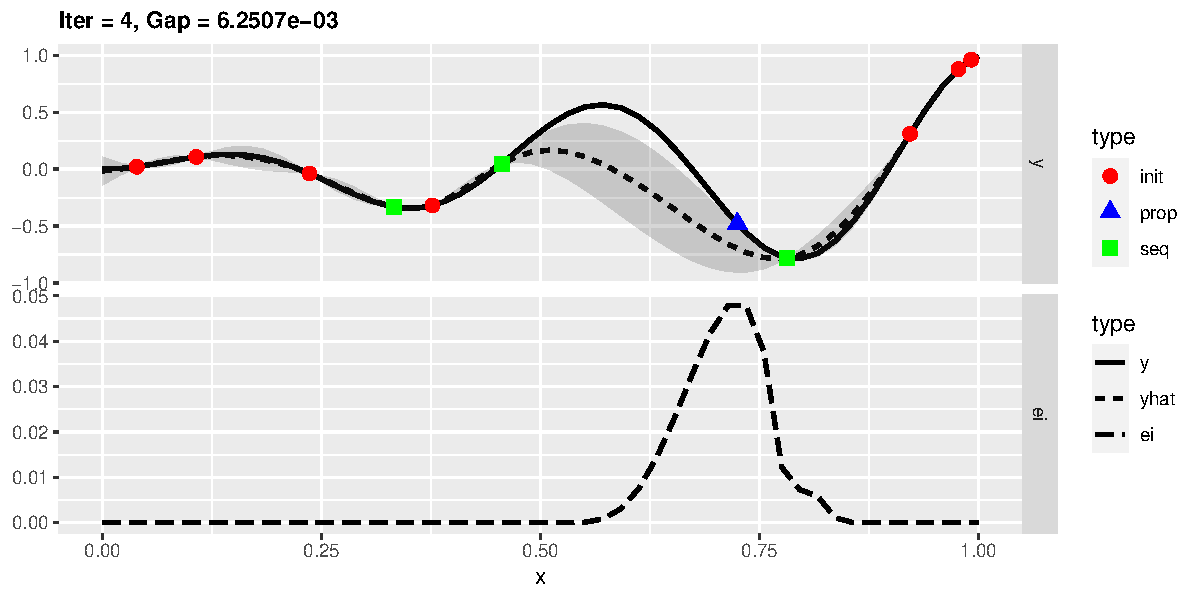
\includegraphics[width=0.95\textwidth]{figure/cart_tuning_ad_4.pdf} 

}



\end{knitrout}
  \begin{footnotesize}
Upper plot: The surrogate model (black, dashed) models the \emph{unknown} relationship between input and output (black, solid) based on the initial design (red points).\\
Lower plot: Mean and variance of the surrogate model are used to derive the expected improvement (EI) criterion. The point that maximizes the EI is proposed (blue point). 
\end{footnotesize}
\framebreak

Since we use the sequentially updated surrogate model predictions of performance to propose new configurations,
we are guided to \enquote{interesting} regions of $\bm{\Lambda}$ and avoid irrelevant evaluations:
  
  \begin{center}
\begin{figure}
% see rsrc/mbo-example.R
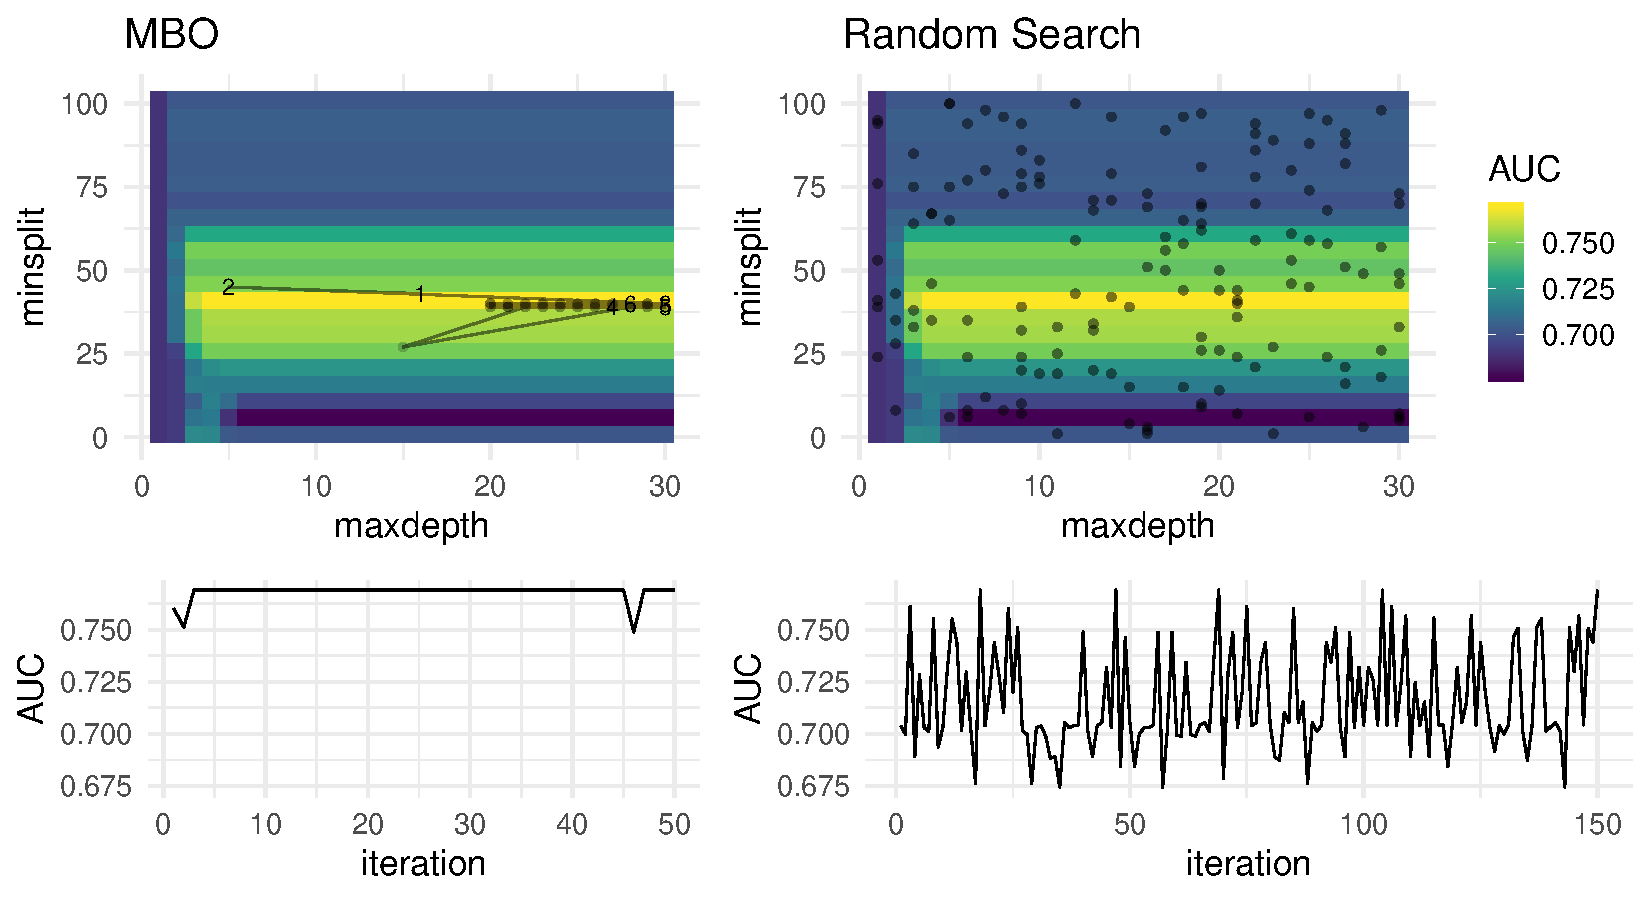
\includegraphics[width=0.7\textwidth]{figure_man/mbo_vs_random.pdf}
\caption{\footnotesize{Tuning tree depth and minimal node size for splits for CART on the \texttt{sonar} data (10-fold CV maximizing AUC). \\
  Left panel: random search, 150 configurations; right panel: MBO, 50 iterations.}}
\end{figure}
\end{center}


\end{vbframe}


\begin{vbframe}{Hyperband}

\begin{itemize}
\item It is extremely expensive to train complex models on large data sets
\item For many configurations, it might be clear early on that further training is not likely to significantly improve the performance
\item More importantly, the relative ordering of configurations (for a given data set) can also become evident early on. 
\item \textbf{Idea:} \enquote{weed out} poor configurations early during training
\item One approach is \textbf{successive halving}: Given an initial set of configurations, all trained for a small initial budget, repeat:
  \begin{itemize}
\item Remove the half that performed worst, double the budget
\item Continue until the new budget is exhausted
\end{itemize}  
\item Successful halving is performed several times with different trade-offs between the number of configurations considered and the budget that is spent on them. 
\end{itemize}

\framebreak 

Only the most promising configuration(s) are trained to completion: 
  
  \begin{center}
\begin{figure}
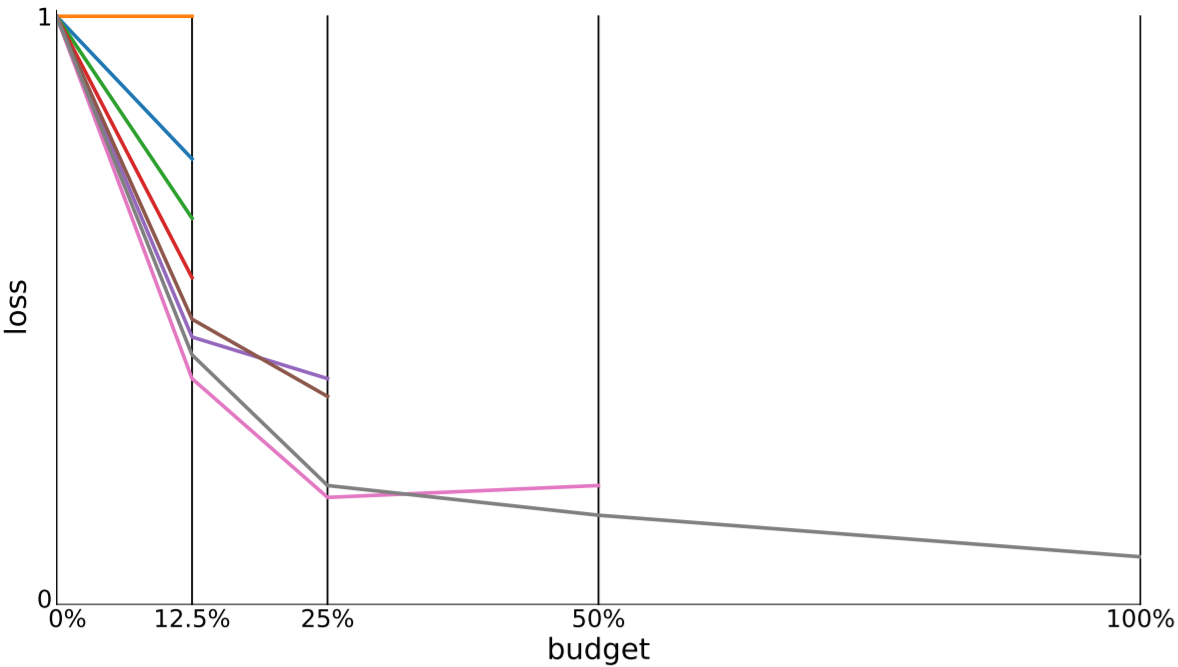
\includegraphics[width=0.8\textwidth]{figure_man/hyperband3.png}
%src: https://www.automl.org/wp-content/uploads/2019/05/AutoML_Book_Chapter1.pdf
\end{figure}
\end{center}
\tiny taken from Hutter, Kotthoff, Vanschoren. \textit{Automated Machine Learning -- Methods, Systems, Challenges}. Springer, 2019. (Fig. 1.3)
\end{vbframe}

\begin{frame}{More tuning algorithms:}

Other advanced techniques besides model-based optimization and the hyperband algorithm are: 
  
  \begin{itemize}
\item Stochastic local search, e.g., simulated annealing
\item Genetic algorithms / CMAES
\item Iterated F-Racing
\item Many more $\ldots$
  \end{itemize}


\end{frame}
\endlecture
\end{document}
